\documentclass[12pt]{article}

% --- Packages ---
\usepackage[utf8]{inputenc}
\usepackage[margin=1in]{geometry}
\usepackage{amsmath, amssymb}
\usepackage{array} 
\usepackage{booktabs}
\usepackage{enumitem}
\usepackage{fancyhdr}
\usepackage{float}
\usepackage{graphicx}
\usepackage{hyperref}
\usepackage{listings}
\usepackage{xcolor}

% --- References ---
% https://www.overleaf.com/learn/latex/Bibliography_management_with_biblatex
\usepackage{biblatex}
\addbibresource{references.bib}

% --- Formatting Setup ---
\hypersetup{
    colorlinks=true,
    linkcolor=blue,
    filecolor=magenta,      
    urlcolor=blue,
}

\title{CSE 554: Assignment 4}
\author{Jack Lowry, Nam Pho, Brett Saiki}
\date{March 13, 2026}

\begin{document}

\pagestyle{fancy}

\fancyhead{} % clear all header fields
\fancyhead[LO]{CSE 554: Group 14}
\fancyhead[CO]{HW4 (Winter 2026)}
\fancyhead[RO]{March 13, 2026}

\fancyfoot{} % clear all footer fields
\fancyfoot[CO]{\thepage}

\maketitle

% --- Section 1: Continuous Batching and Chunked Prefill ---
\section{Continuous Batching and Chunked Prefill}

\begin{enumerate}[label=\textbf{Q\arabic*.}]
    \item % --- Section 1, Question 1 ---
    Implement the continuous batching in the files \texttt{Section1/continous\_engine.py} and \texttt{Section1/continuous\_scheduler.py}.
    
    With batch size 10, input length following a uniform distribution between [1,10], output length following a uniform distribution between [1, 128], profile the end-to-end execution time of naive scheduling and continuous batching serving 100 requests. What is the speedup over naive scheduling? \\

    We observe a speedup of approximately $1.5\times$ over naive scheduling. \\

    \item % --- Section 1, Question 2 ---
    Implement chunked prefill in the files
    \texttt{Section1/chunked\_engine.py} and \texttt{Section1/chunk\allowbreak ed\_scheduler.py}.
    Control the maximum token batch size to be 512 in each iteration.

    \begin{enumerate}
        \item With the input length following a lognormal distribution with $\mu = 6$, $\sigma = 0.7$, and the output length following a uniform distribution between [1, 512], profile the end-to-end execution time of the chunked prefill solution. How does it compare with continuous batching?  \\

        We observe a speedup of approximately $1.347\times$ without chunked prefill. \\

        \item Compare the iteration time of continuous batching and chunked prefill by plotting them as scatter plots, with iteration id as the x-axis. What is the difference? \\

        Continuous batching has a mostly consistent per-iteration time with a scattering of high latency requests. Chunked prefill has an initial period of high-latency requests before the time suddenly drops and consistently trends lower; unlike continuous batching there are few outliers in the data. Figure \ref{fig:s1:cont_vs_chunk} shows these trends.
        \begin{figure}[H]
            \centering
            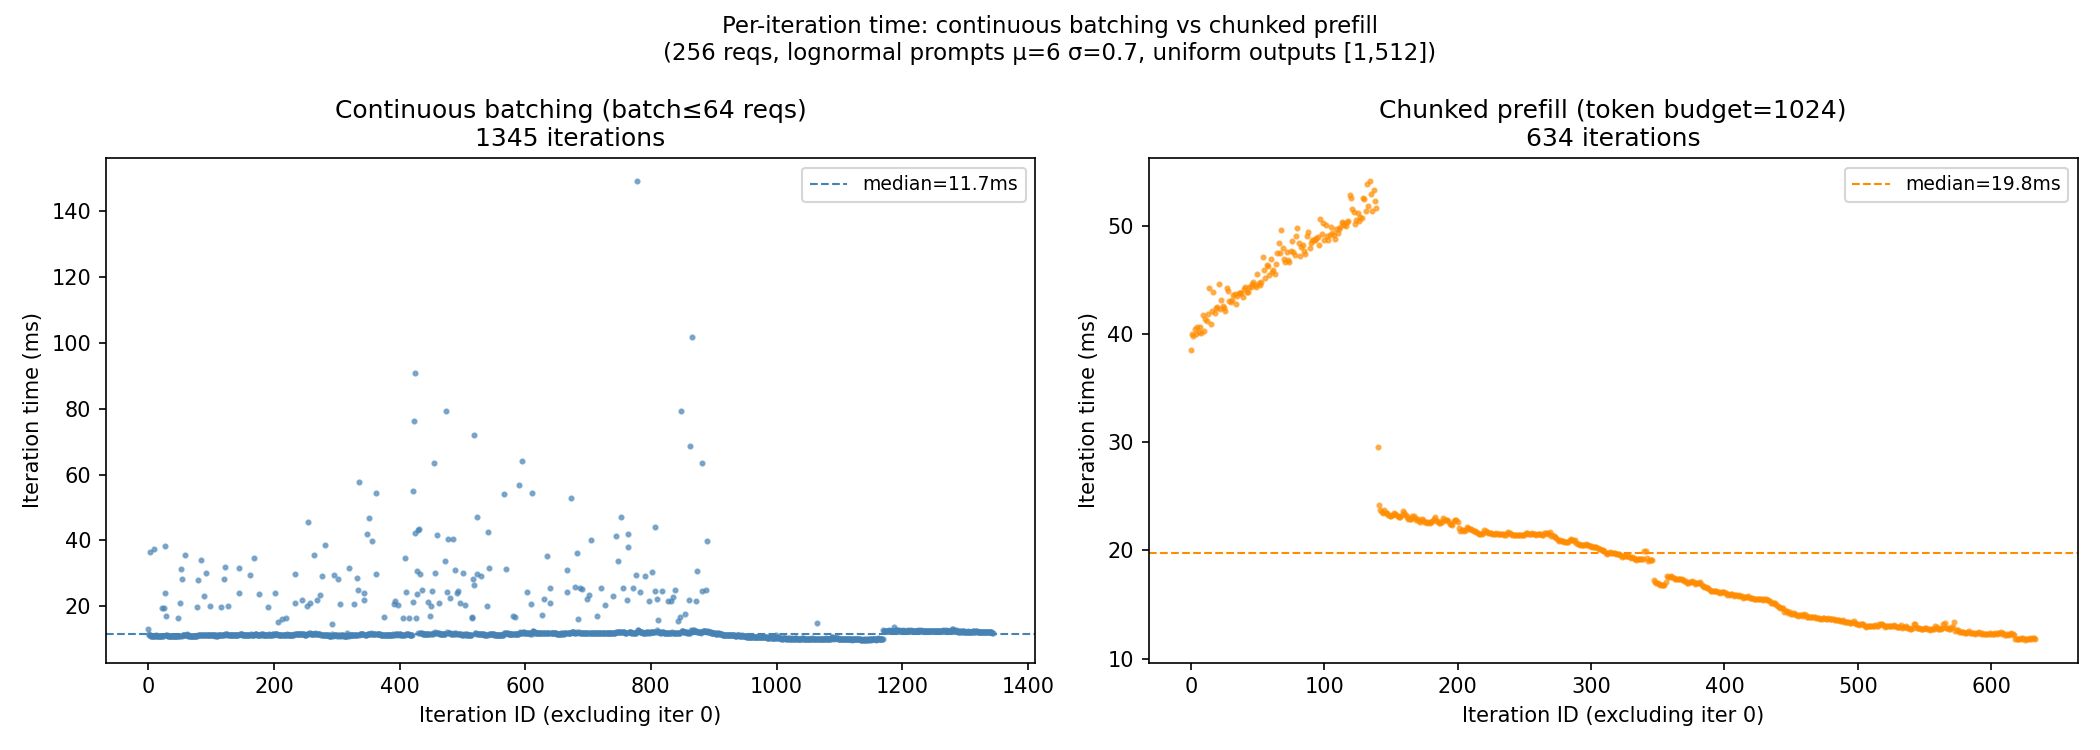
\includegraphics[width=1\linewidth]{fig/iter_time_scatter.png}
            \caption{Continuous batching versus chunked prefill.}
            \label{fig:s1:cont_vs_chunk}
        \end{figure}

    \end{enumerate}

    \item % --- Section 1, Question 3 ---
    \begin{enumerate}
        \item Profile vLLM performance with llama-3.2-1B, with input length 512, output length 512, and request number 100. You can use the benchmark script \href{https://docs.vllm.ai/en/stable/cli/bench/serve/}{here}.  \\

Start the vLLM server as a background process.
\begin{verbatim}
vllm serve /local1/cse554/models/meta-llama/Llama-3.2-1B/ \
    --port 1234 &
\end{verbatim}
Query the server using the benchmark settings.
\begin{verbatim}
vllm bench serve \
    --model /local1/cse554/models/meta-llama/Llama-3.2-1B/ \
    --dataset-name random \
    --input-len 512 \
    --output-len 512 \
    --num-prompts 100 \
    --port 1234
\end{verbatim}
Condensed output from profiling.
\begin{verbatim}
============ Serving Benchmark Result ============
Successful requests:                     100       
Failed requests:                         0         
Benchmark duration (s):                  13.97     
Total input tokens:                      51100     
Total generated tokens:                  51200     
Request throughput (req/s):              7.16      
Output token throughput (tok/s):         3663.89   
Peak output token throughput (tok/s):    7900.00   
Peak concurrent requests:                100.00    
Total token throughput (tok/s):          7320.62   
---------------Time to First Token----------------
Mean TTFT (ms):                          4252.25   
Median TTFT (ms):                        3502.35   
P99 TTFT (ms):                           6871.52   
-----Time per Output Token (excl. 1st token)------
Mean TPOT (ms):                          18.80     
Median TPOT (ms):                        20.28     
P99 TPOT (ms):                           21.31     
---------------Inter-token Latency----------------
Mean ITL (ms):                           18.80     
Median ITL (ms):                         14.03     
P99 ITL (ms):                            59.63     
==================================================    
\end{verbatim}

        \item Profile your own chunked prefill performance with input length 512, output length 512, and 100 requests. How does that compare with vLLM? Which part (attention, FFN, other small kernels, overheads, etc) of vLLM is faster than your own implementation? \\

        Our chunked prefill performance was slower than vLLM. Chunked prefill returns tokens faster but vLLM has a higher overall throughput. Presumably this is due to the use of non-contiguous memory that is allocated as needed in Paged Attention of vLLM versus the simpler approach to addressing compute ``bubbles'' by chunked prefill with worst case memory allocation up front.

    \end{enumerate}
    
\end{enumerate}

% --- Section 2: Parallelism ---
\section{Parallelism}

\begin{enumerate}[label=\textbf{Q\arabic*.}]
    \item % --- Section 2, Question 1 ---
    \begin{enumerate}
        \item Profile the network bandwidth utilization of PyTorch’s all-reduce collective communication by running the script in \texttt{Section2/profile\_allreduce.py}.

        \begin{figure}[H]
            \centering
            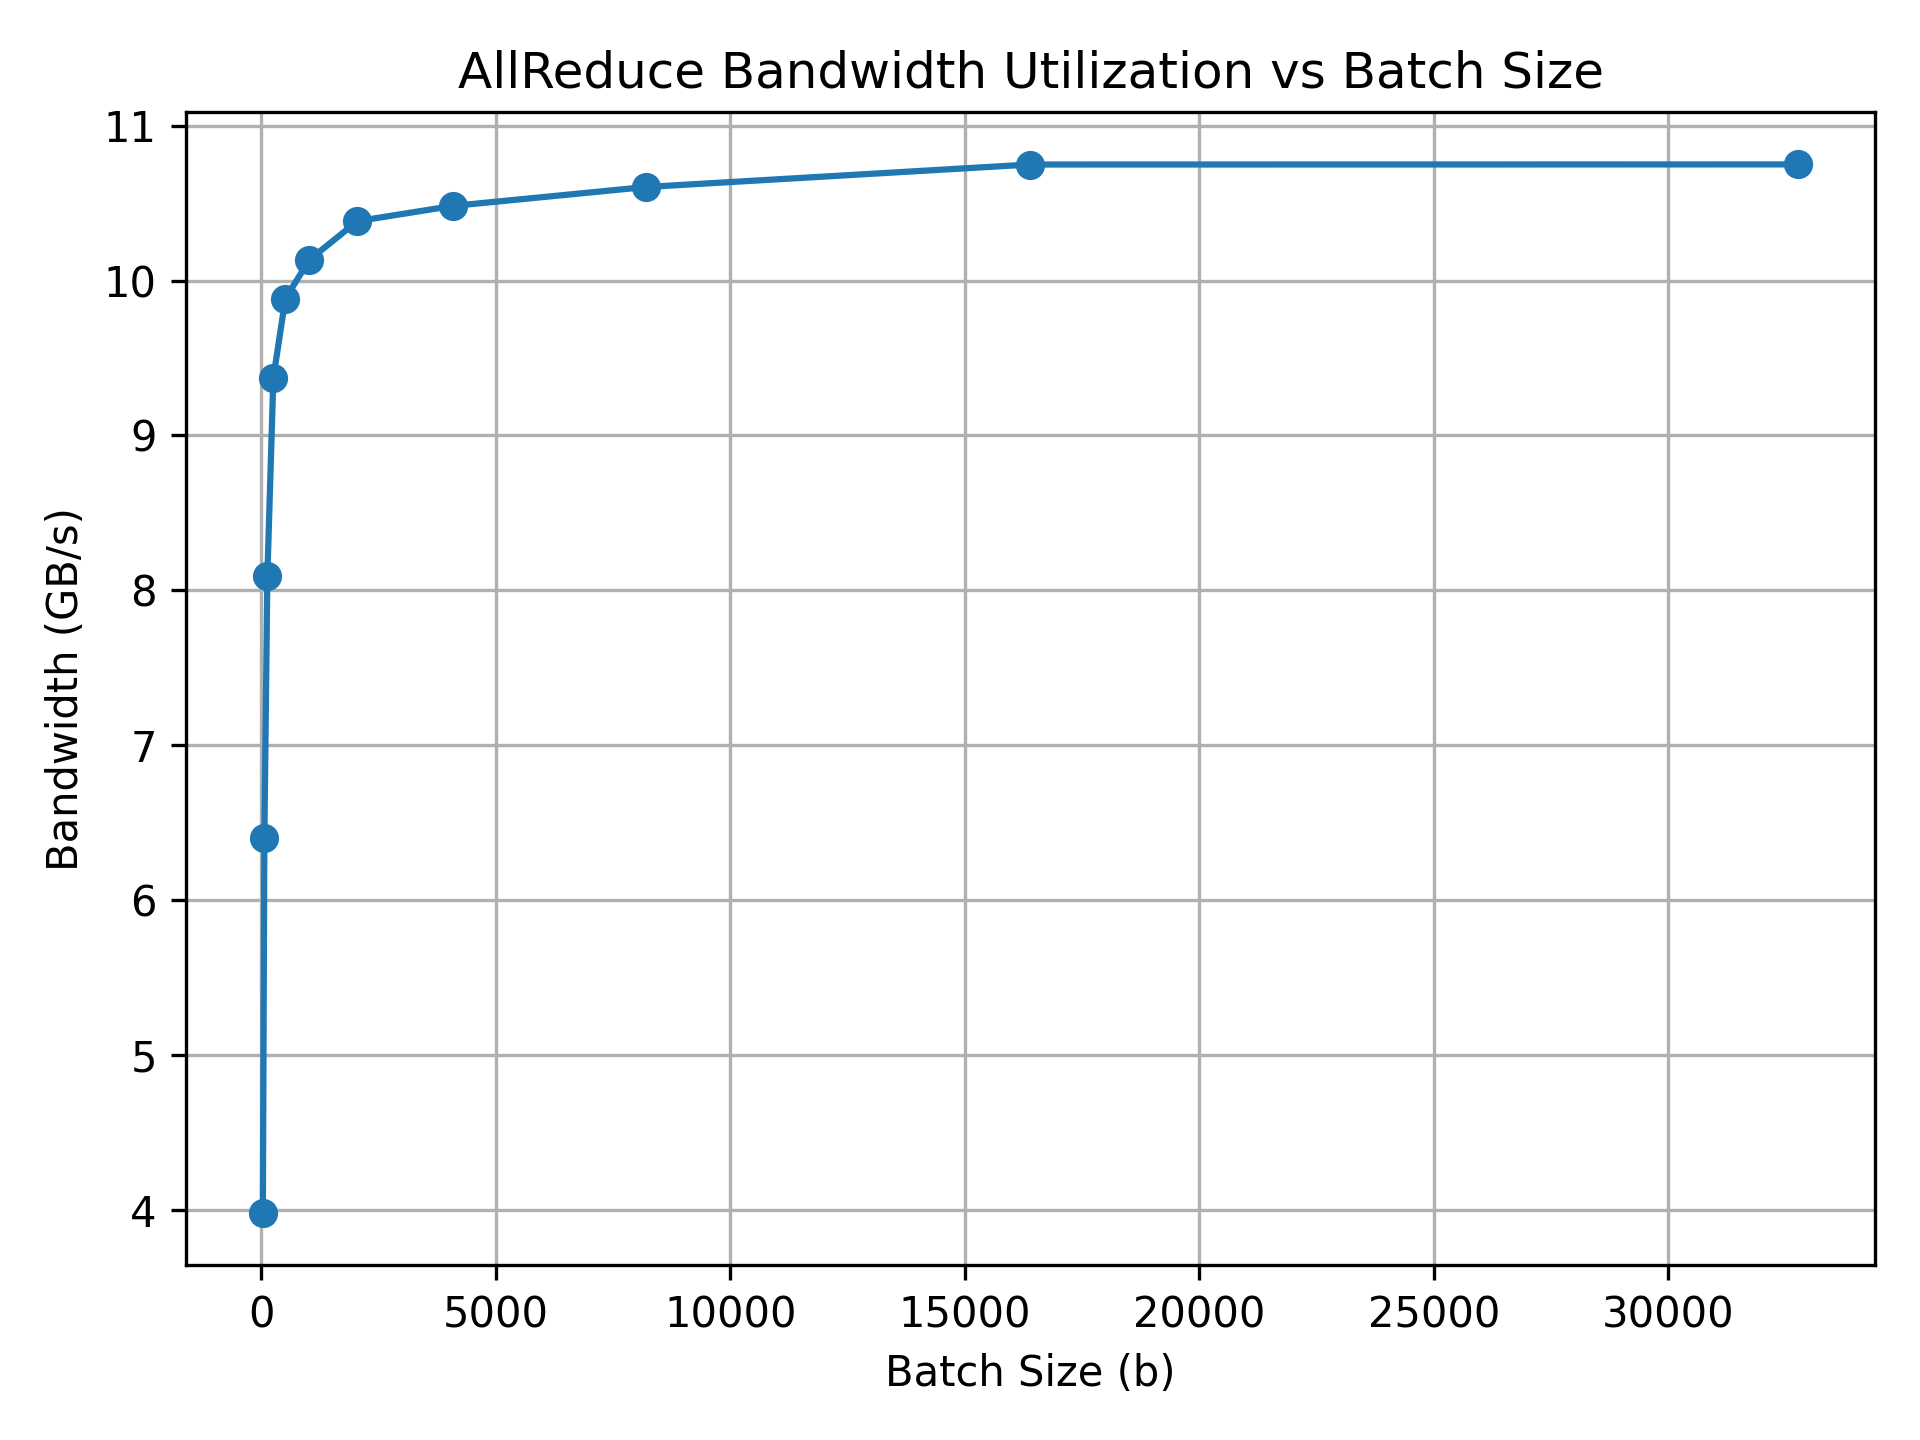
\includegraphics[width=0.55\linewidth]{fig/profile_allreduce.png}
            \caption{Profiling the scalability of all-reduce operations in PyTorch.}
            \label{fig:allreduce}
        \end{figure}
        
        What trend do you observe from the bandwidth utilization figure generated? How does the achieved network bandwidth utilization compare to the theoretical network bandwidth? \\

        The trend we observed is that PyTorch all reduce quickly saturates the PCIe interconnect and that the network becomes the bottleneck for further scaling. From the \texttt{nvidia-smi} topology output below, each pair of GPUs communicates over PCIe gen 3.0 (8 GT/s) and operates with x16 throughput leading to a theoretical bandwidth of \boxed{ \textbf{16 GB/s} } between GPU pairs. \\
        
        To calculate theoretical network bandwidth, use \texttt{nvidia-smi topo -m} to output the network topology of the cluster.
        
\begin{verbatim}
$ nvidia-smi topo -m
        GPU0    GPU1    GPU2    GPU3    GPU4    GPU5    GPU6    GPU7    NIC0    CPU Affinity      NUMA Affinity   GPU NUMA ID
GPU0     X      PIX     PXB     PXB     PXB     PXB     PIX     PIX     SYS     0-1     0N/A
GPU1    PIX      X      PXB     PXB     PXB     PXB     PIX     PIX     SYS     0-1     0N/A
GPU2    PXB     PXB      X      PIX     PIX     PIX     PXB     PXB     SYS     0-1     0N/A
GPU3    PXB     PXB     PIX      X      PIX     PIX     PXB     PXB     SYS     0-1     0N/A
GPU4    PXB     PXB     PIX     PIX      X      PIX     PXB     PXB     SYS     0-1     0N/A
GPU5    PXB     PXB     PIX     PIX     PIX      X      PXB     PXB     SYS     0-1     0N/A
GPU6    PIX     PIX     PXB     PXB     PXB     PXB      X      PIX     SYS     0-1     0N/A
GPU7    PIX     PIX     PXB     PXB     PXB     PXB     PIX      X      SYS     0-1     0N/A
NIC0    SYS     SYS     SYS     SYS     SYS     SYS     SYS     SYS      X

Legend:

  X    = Self
  SYS  = Connection traversing PCIe as well as the SMP interconnect between NUMA nodes (e.g., QPI/UPI)
  NODE = Connection traversing PCIe as well as the interconnect between PCIe Host Bridges within a NUMA node
  PHB  = Connection traversing PCIe as well as a PCIe Host Bridge (typically the CPU)
  PXB  = Connection traversing multiple PCIe bridges (without traversing the PCIe Host Bridge)
  PIX  = Connection traversing at most a single PCIe bridge
  NV#  = Connection traversing a bonded set of # NVLinks

NIC Legend:

  NIC0: mlx5_0
\end{verbatim}

        \item You are given the transformer implementation for Lama-3.2-1B shown in class in \texttt{Section2/transformer-w3l1.py}. Now we want to extend this implementation to support running Lama-3.2-1B using tensor parallelism of degree 2. Implement the tensor-parallel version of the attention block in \texttt{Section2/transformer-tp2.py}. Note that Q/K/V projection weights are split by head, and the output projection weight is split by row (refer to Lecture 14, Slide 32). \\


        \item Implement the tensor-parallel version of the feed-forward network in \texttt{Section2/tr\allowbreak ansformer-tp2.py}. Note that the up and gate weights are split by column, and the down projection weight is split by row (refer to Lecture 14, Slide 31). You are expected to see the same output as running the original single-GPU implementation in \texttt{Section2/transformer-w3l1.py}. Run \texttt{torchrun --nproc-per-node=2 Section2/transformer-tp2-answer.py} to test your implementation. This will set up ranks and world size for 2 GPUs automatically. \\

        \item Profile the generation time for the tensor-parallel version of the Lama-3.2-1B implementation and compare it with the generation time for the original implementation. Is the generation time faster for the tensor-parallel version? If so, what are the reasons that lead to the speed-up? If not, what are the reasons causing the overheads? \\

        The tensor-parallel version of Lama-3.2-1B takes on average 2.92 seconds for over 10 runs, while the single-GPU version takes on average 3.17 seconds over 10 runs, achieving an approximately $10\%$ speedup. The reasons for this speedup is that each seperate GPU can achieve a higher throughput seperately than if the same operations were run on a single GPU. Additionally, since batch size is 1 here, communication costs are relatively cheap, so the all-reduce operations do not significantly slow down computation.
    
        

    \end{enumerate}
\end{enumerate}

\printbibliography

\end{document}